\documentclass{article}
\usepackage{graphicx,fancyhdr,amsmath,amssymb,amsthm,subfig,url,hyperref}
\usepackage[margin=1in]{geometry}
\usepackage{xltxtra}
\usepackage{xgreek}
\usepackage{amsfonts}
\usepackage{amssymb}
\usepackage{amsmath}
\usepackage{graphicx}
\usepackage{listings}


\usepackage{caption}
\usepackage{ subfig}
%\setmainfont[Mapping=tex-text]{Times New Roman}
\setmainfont{GFS Artemisia}
%----------------------- Macros and Definitions --------------------------
% FILL THIS OUT
\newcommand{\studentname}{Νικόλαος Ζαρίφης}
\newcommand{\suid}{03112178}
\newcommand{\exerciseset}{Τρίτη εργαστηριακή Άσκηση}
% END



\renewcommand{\theenumi}{\bf \Alph{enumi}}

%\theoremstyle{plain}
%\newtheorem{theorem}{Theorem}
%\newtheorem{lemma}[theorem]{Lemma}

\fancypagestyle{plain}{}
\pagestyle{fancy}
\fancyhf{}
\fancyhead[RO,LE]{\bfseries\large NTUAthens}
\fancyhead[LO,RE]{\bfseries\large Δίκτυα επικοινωνιών}
\fancyfoot[LO,RE]{\bfseries\large \studentname: nick.zarifis@hotmail.com}
\fancyfoot[RO,LE]{\bfseries\thepage}
\renewcommand{\headrulewidth}{1pt}
\renewcommand{\footrulewidth}{1pt}

\graphicspath{{figures/}}

%-------------------------------- Title ----------------------------------

\title{Δίκτυα επικοινωνιών \\ \exerciseset}
\author{\studentname \qquad  ID: \suid}

%--------------------------------- Text ----------------------------------

\begin{document}
\maketitle

\section*{Ερωτήσεις 1}
 Το σχήμα που προέκυψε είναι το ακόλουθο:\\
\begin{figure}[ht!]
	\centering
\subfloat[Δυκτιό]{{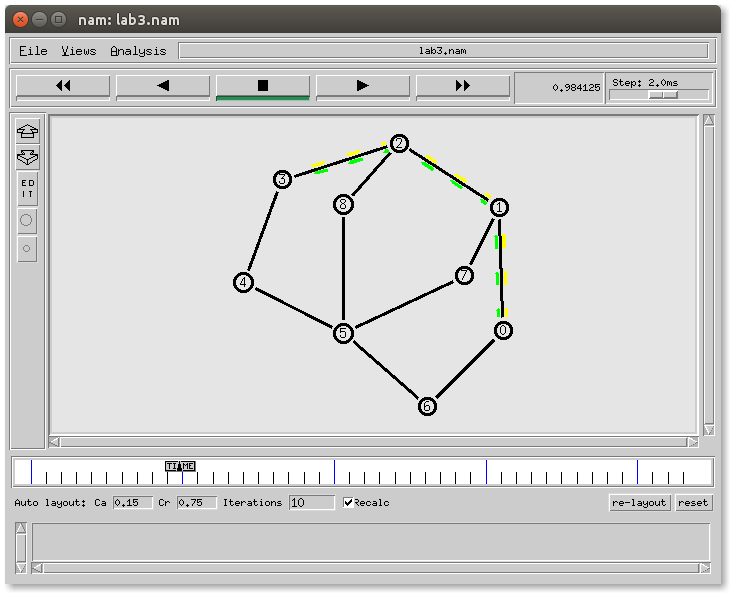
\includegraphics[height=150pt,width=150pt]{ex1nam}}
}
   \qquad
\subfloat[without packetSize]{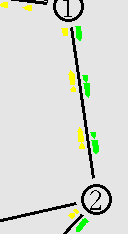
\includegraphics[height=150pt,width=120pt]{ex1last2}}\caption{nam of ex 1}

\end{figure} \\
\begin{itemize}
\item \textbf{Ποια διαδρομή ακολουθούν τα πακέτα;}\\
Τα πράσινα πακέτα ξεκινάνε από τον κόμβο 0 κι πάνε στον 3 ακολουθώντας την διαδρομή 0-1-2-3. Ενώ τα κίτρινα πάνε από τον 3 στον 0 από την διαδρομή 3-2-1-0.
\item
\textbf{Ελέγξτε αν η ροή των πακέτων και από τις δυο πλευρές ακολουθεί τη διαδρομή με τα λιγότερα βήματα.}\\
Βλέπουμε ότι κι οι 2 διαδρομές έχουν 3 βήματα η οποία είναι η διαδρομή με τα λιγότερα βήματα. Εκτελώντας έναν αλγόριθμο BFS στον γράφο αφού δεν έχουμε βάρος μας επιβεβαιώνει το αποτέλεσμά μας.
\item
\textbf{Υπάρχει συντομότερη διαδρομή από αυτήν που ακολουθούν, όσον αφορά τη συνολική καθυστέρηση κάθε ροής; }\\
Η διαδρομή που έχουμε είναι η καλύτερη και από την μεριά της καθυστέρησης έχοντας συνολική 60ms.Η μόνη εναλλακτική  περνάει από το  διαδρομή 1-7-5 και όποια κατεύθυνση αν πάρει θα έχει περισσότερο καθυστέρηση.Ο αλγόριθμος του Dijkstra  σε τέτοιες περιπτώσεις μας επιβεβαιώνει το αποτέλεσμα.
\item
\textbf{Ποιος είναι ο ρόλος των εντολών \$udp0 set packetSize\_ 1500 και \$udp3 set packetSize\_ 1500; Τι παρατηρείτε στις ροές των πακέτων αν αφαιρεθούν οι γραμμές
	αυτές από τον κώδικα της προσομοίωσης; }\\
Όπως βλέπουμε στην εικόνα στέλνει 2 πακέτα. Αυτό συμβαίνει γιατί συμφωνά με το documation ορίζει ως default value το size=1000Β  άρα ότι είναι μεγαλύτερο το σπάει σε κομμάτια. 

\end{itemize}



\section*{Ερωτήσεις 2}
\begin{figure}[ht!]
	\centering
	\subfloat[Static]{{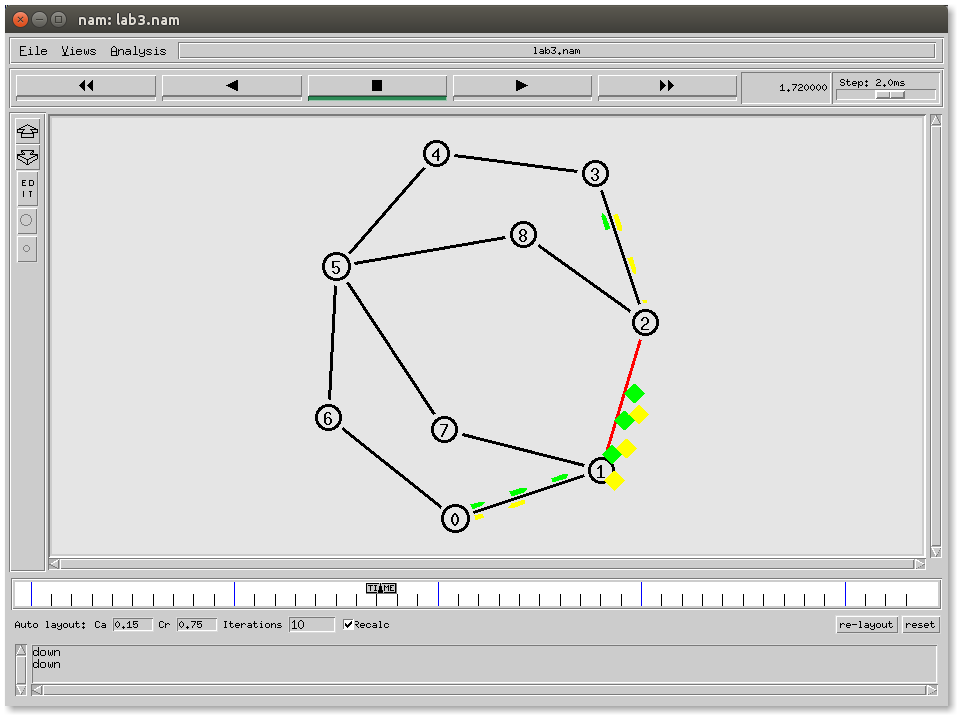
\includegraphics[height=150pt,width=150pt]{staticloss}}
	}
	\qquad
	\subfloat[Dynamic]{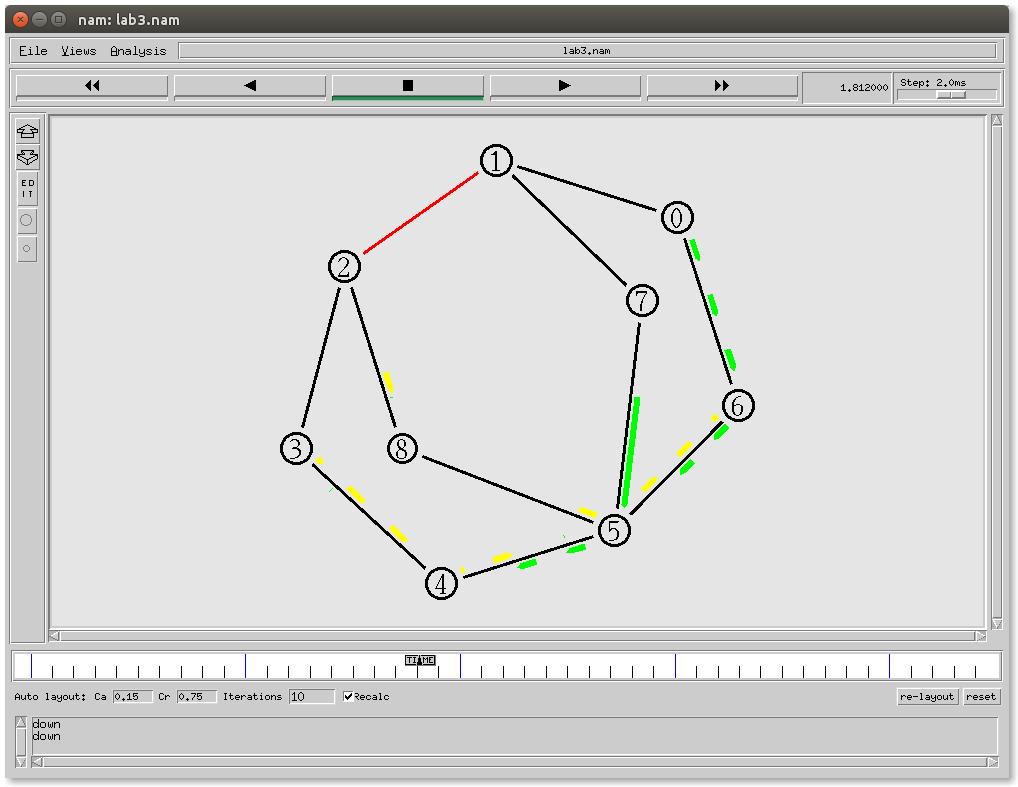
\includegraphics[height=150pt,width=120pt]{dynamic}}\caption{nam of ex 2}
	
\end{figure} 	
\begin{itemize}
\item
\textbf{Εξηγήστε γιατί, με τη στατική δρομολόγηση, οι κόμβοι εξακολουθούν να στέλνουν
	πακέτα και μετά τη διακοπή της ζεύξης. } \\
Ο λόγος είναι ότι το δίκτυο μας δεν διαθέτη κάποιον τρόπο για να ανακαλύψει ότι η ζεύξη έπεσε, όποτε συνεχίζει να στέλνει σαν να μην συνέβηκε τίποτα.
\item \textbf{Τα πακέτα που χάθηκαν, θα ξαναμεταδοθούν από τους αντίστοιχους κόμβους, όταν
	επανέλθει η σύνδεση;}\\ Όχι , γιατί όπως είπαμε οι πομποί δεν καταλαβαίνουν πως έπεσε η ζεύξη.
\item \textbf{ Τι παρατηρείτε όταν γίνεται διακοπή ζεύξης και έχουμε δυναμική δρομολόγηση;
	Περιγράψτε με απλά λόγια τη διαδικασία που λαμβάνει χώρα στο animation.Συμπίπτει η
	αρχική με τη μόνιμη διαδρομή δρομολόγησης για τις δύο ροές κατά τη διάρκεια της
	διακοπής; }\\
Όταν η ζεύξη πέσει τότε το rtproto θα ειδοποιήσει το σύστημα κι θα βρεθεί μια νέα διαδρομή για να στείλει τα πακέτα όπου θα είναι η πιο σύντομη. Αλλά τα πακέτα που είχε στείλει πριν την νέα μόνιμη διαδρομή κι έχουν φτάσει στον κόμβο 1 και στον 2 αντίστοιχα, στέλνονται στον 7-5 και 8-5 . Και απο εκεί ακολουθούν την κοινή διαδρομή με τα άλλα πακέτα που είναι η 0-6-5-4-3.Τέλος όταν ξαναναίβει η ζεύξη το rtproto ενημερώνει την διαδρομή κι στέλνονται τα υπόλοιπα πακέτα από εκεί.
\item \textbf{Με βάση το animation, προσδιορίστε για κάθε ροή τη χρονική στιγμή όπου παρατηρείται
	η μόνιμη διαδρομή δρομολόγησης κατά τη διάρκεια διακοπής}\\
Βλέπουμε πως ταυτόχρονα κι στους δυο πομπούς ακολουθούν την μόνιμη διαδρομή πέριπου στο 1.85s.Αυτό γίνεται γιατί τότε πέρνουν την πληροφορία απο το rtproto.
\item \textbf{Για ποιο λόγο τα πακέτα ακολουθούν τις συγκεκριμένες διαδρομές αφότου πέσει η
	σύνδεση, στην αρχική και τη μόνιμη κατάσταση; }\\
Αυτό συμβαίνει επειδή είναι η ελάχιστη διαδρομή από θέμα καθυστερήσεις ανάμεσα στους δύο κόμβους.Στην αρχική κατάσταση κοιτάει από τον κόμβο 1,2 και μετά απο τους κόμβους 0,3.
\item \textbf{ Θα μπορούσαν να δρομολογηθούν από άλλους κόμβους; }\\ Ναι γίνεται υπάρχουν κι άλλες διαδρομές όπως βλέπουμε αλλά δεν είναι ελάχιστες.
\item \textbf{Ποιος από όλους τους κόμβους καθορίζει από ποια διαδρομή θα προωθηθούν κάθε φορά
	τα πακέτα; }\\ Πάντα αποφασίζει η πηγή αλλά πριν την μόνιμη κατάσταση αποφασίζουν οι κόμβοι που έχουν πακέτα εκείνη την στιγμή δηλαδή στην περίπτωση μας ο 1,2 .
\end{itemize}
\section*{Ερωτήσεις 3}
\begin{figure}[ht!]
	\centering
	\subfloat[Before]{{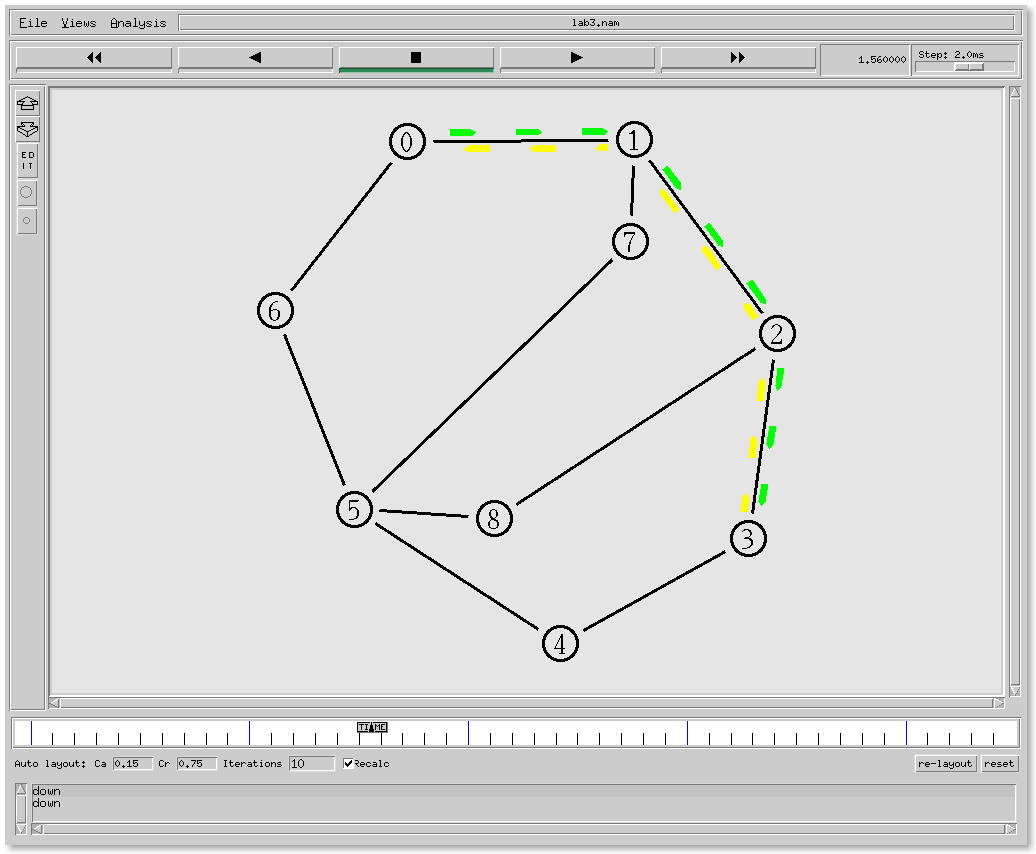
\includegraphics[height=150pt,width=150pt]{ex3be}}
	}
	\qquad
	\subfloat[After]{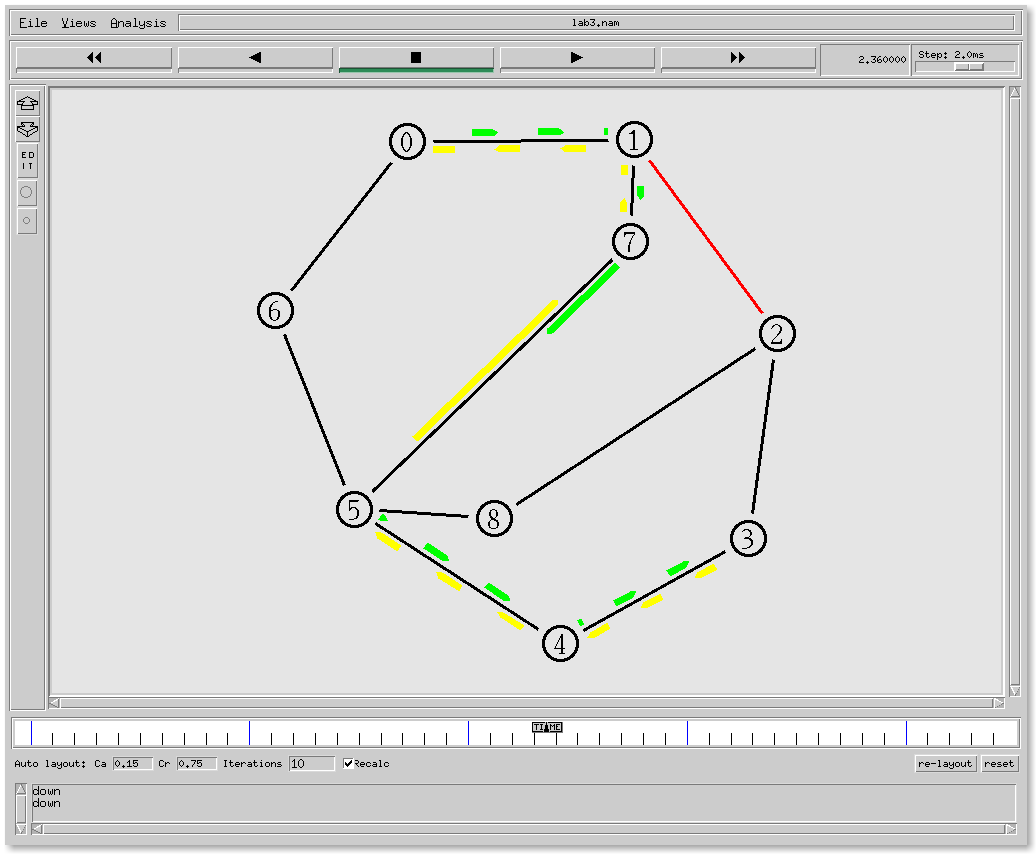
\includegraphics[height=150pt,width=120pt]{ex3a}}\caption{nam of ex 3}
	
\end{figure} 	
\begin{itemize}
	\item
	\textbf{Ποιες διαδρομές ακολουθούν τα πακέτα πριν, κατά τη διάρκεια και μετά την πτώση της
		σύνδεσης για τις δύο ροές;}\\
	Πριν την πτώση ακολουθούν την ίδια διαδρομή με πριν. Αλλά όταν πέσει η γραμμή τα πακέτα προτειμόυν  την διαδρομή 0-1-7-5-4-3 γιατί έχει το μικρότερο κόστος.
	\item
	\textbf{Για ποιον λόγο τα πακέτα ακολουθούν τις συγκεκριμένες διαδρομές; }
	\\ Έχουν κι τα 2 το ελάχιστο κόστος. Όταν πέσει η γραμμή έχει κόστος 15 κι όταν δεν έχει πέσει έχει 12.Υπολογίζοντας την διαδρομή που ακολουθούσε πριν όταν είχε πέσει η γραμμή ,τώρα έχει κόστος 16.
	\item
	\textbf{Θα μπορούσαν να δρομολογηθούν από άλλους κόμβους;}\\
	Ναι γίνεται αφού υπάρχουν κι άλλες διαδρομές αλλά δεν έχουν το λιγότερο κόστος.
	\item
	\textbf{Μετά την αποκατάσταση της ζεύξης μεταξύ των κόμβων “1” και “2”, προσδιορίστε με
		βάση το animation τη χρονική στιγμή όπου παρατηρείται η μόνιμη διαδρομή
		δρομολόγησης για κάθε ροή. }\\ Όταν ανέβει η γραμμή κι οι δύο ροές παίρνουν την μόνιμη κατεύθυνση στα 2.8s.
	\item \textbf{Πριν(?) την αποκατάσταση της ζεύξης μεταξύ των κόμβων “1” και “2”, προσδιορίστε με
		βάση το animation τη χρονική στιγμή όπου παρατηρείται η μόνιμη διαδρομή
		δρομολόγησης για κάθε ροή. } \\ Η πρώτη ροή πέρνει την μόνιμη κατασταση κατευθείαν αφού η διαδρομή αυτή περνά απο τον κόμβο 1. Η αλλή ροή όμως αργεί λίγο γιατί πρέπει να στείλει τα πακέτα από τον κόμβο 2 που έχουν μείνει κι δεν ανείκει στην ελάχιστη διαδρομή. Περίπυο 1.85s.
	\item \textbf{Ποιος είναι ο ρόλος της εντολής Agent/rtProto/Direct set preference\_ 200;
		Τι παρατηρείτε στη δρομολόγηση των πακέτων αν αφαιρεθεί η εντολή αυτή από τον
		κώδικα της προσομοίωσης; Αιτιολογείστε γιατί συμβαίνει αυτό. } \\	
	Η εντολή αυτή έχει ως αποτέλεσμα να κρατάει πληροφορίες για την σύνδεση με τους γειτονικούς κόμβους,όπως επίσης από DV έχει κι όλες τις πιθανές διαδρομές.Και έτσι όταν διακοπεί η  διαδρομή μπορεί να βρει μια νέα διαδρομή.Έτσι βλέπουμε πως όταν αφαιρούμε την εντολή κάνει περισσότερο χρόνο να αποφασίσει την νέα διαδρομή.Γιατί πρέπει πρώτα να ενημερωθεί ο κόμβος 0 (ή 3) κι να καθορίσει την νέα διαδρομή σε αντίθεση με όταν είχαμε την εντολή κι καθόριζε ο κόμβος πριν την γραμμή που έπεσε.
\end{itemize}
\lstinputlisting{ex3lab3.tlc}
\section*{Ερωτήσεις 4}
\begin{figure}[ht!]
	\centering
	\subfloat[CBR]{{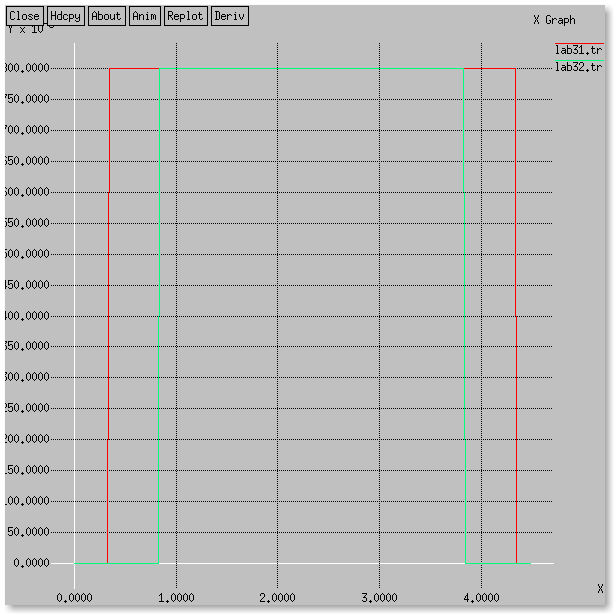
\includegraphics[height=150pt,width=150pt]{x1}}
	}
	\qquad
	\subfloat[Expomential]{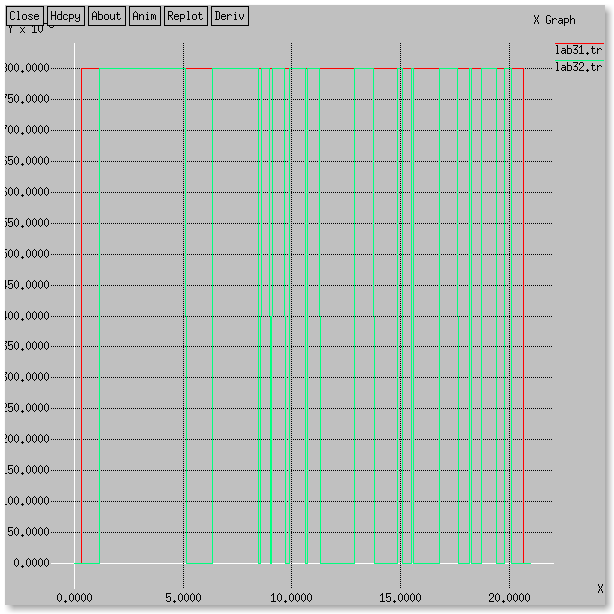
\includegraphics[height=150pt,width=120pt]{xgraph3}}\caption{xgraph}
	
\end{figure}
\begin{itemize}
	\item \textbf{Ποιος είναι ο μέγιστος ρυθμός μετάδοσης που επιτυγχάνεται για τις δύο περιπτώσεις
		κίνησης, βάσει των γραφικών παραστάσεων που σχεδιάσατε; } \\ Όπως βλέπουμε κι στις δύο περιπτώσεις έχουμε μέγιστο ρυθμό μετάδοσης 0.8Mbits/s
	\item \textbf{Αιτιολογείστε τις μέγιστες τιμές που προσδιορίσατε παραπάνω, χρησιμοποιώντας τις
		παραμέτρους που θέσατε για τη διαμόρφωση των δύο πηγών κίνησης (CBR και
		Exponential).}\\Όταν έχουμε CBR έχουμε από τύπους που έχουμε χρησιμοποιείσει σε παλιότερες ασκήσεις έχουμε : $\frac{packets}{rate}=\frac{1500}{0.015}=10^5bytes/s=0.8*10^6Bits/s=0.8Mbits/s$. Τώρα όταν έχουμε Expomential έχουμε ρυθμίσει manualy τον ρυθμό απο την εντολή rate=800k $\rightarrow$ 0.8MBits/s.
	\item \textbf{Υπολογίστε το πλήθος των bytes που λαμβάνονται επιτυχώς στον προορισμό για κάθε
		ροή, θεωρώντας ότι και οι δύο ροές ολοκληρώνονται σε χρόνο t=20+(a/10)sec, όπου a τα
		δύο τελευταία ψηφία του αριθμού μητρώου σας. }
	Για α=78 έχουμε t=27.8s.Προσθέτοντας μεταβλητές που να υπολογίζουν τα συνολικά bytes που λαμβάνονται έχουμε ως αποτέλεσμα από 0 με προορισμό 3 έχουμε 2755500Bytes κι απο 3 με 0 έχουμε 1588500Bytes.
	
\end{itemize}

\lstinputlisting{lab3.tlc}


\end{document}